\documentclass{article}
\usepackage[utf8]{inputenc}
\usepackage{amsmath, amssymb}
\usepackage{graphicx}
\usepackage{hyperref}

\title{SICNN: Smooth Information Criterion Neural Networks for Sparse Neural Modeling}
\author{Aliaksandr Hubin, Andrew McInerney}
\date{\today}

\begin{document}
\maketitle

\begin{abstract}
Smooth Information Criterion Neural Networks (SICNNs) provide a deterministic, smooth-$L_0$ approach to sparse neural network training in \texttt{torch}. The current implementation optimizes neural weight means directly and adds a Smooth Information Criterion (SIC) penalty to the data-fit loss. Sparsity is induced through the surrogate
\[
\phi_\epsilon(w)=\frac{w^2}{w^2+\epsilon^2},
\]
with an epsilon-telescope that progressively sharpens the approximation to an $L_0$ count. The package supports feed-forward networks with optional input-skip connections for feature selection, convolutional layers with the same smooth weight penalty, sparse-path inference for feed-forward architectures, local gradient explanations, and frequentist uncertainty approximations for those explanations. The method is best viewed as a BIC-calibrated neural pruning framework rather than as a direct application of classical BIC theory to a regular parametric model.
\end{abstract}

\section{Introduction}
Modern high-dimensional datasets often require models that are predictive while still revealing which inputs and pathways are being used. Classical neural networks are typically dense and difficult to interpret, while exact subset selection over neural subnetworks is combinatorial. SICNN addresses this by replacing discrete inclusion indicators with a differentiable approximation to the number of nonzero weights. The resulting objective can be optimized with standard gradient-based tools while encouraging weights to collapse toward zero.

The package is related historically to Latent Binary Bayesian Neural Networks (LBBNNs), but the current \texttt{train\_SICNN()} implementation is deterministic and SIC-based. It does not expose a variational-inclusion training criterion or a KL-divergence objective. Instead, it stores trainable weight means in \texttt{SICNN\_Linear} and \texttt{SICNN\_Conv2d} modules, applies the smooth $L_0$ penalty to those weight tensors, and then derives sparse inference paths by thresholding the trained weights.

\section{Current Implementation}
\subsection{Network Classes}
The main feed-forward model is \texttt{SICNN\_Net}. For layer sizes
\[
(p,h_1,\ldots,h_L,o),
\]
the model creates \texttt{SICNN\_Linear} layers followed by an output layer. When \texttt{input\_skip = TRUE}, the original input vector is concatenated into every hidden layer after the first and also into the output layer. These skip connections allow the final sparse graph to represent both direct effects and hidden nonlinear transformations of the input features.

The package also includes \texttt{SICNN\_Conv2d} and a simple \texttt{SICNN\_ConvNet} wrapper for image-style classification. Convolutional layers use the same trainable \texttt{weight\_mean} tensors and the same smooth $L_0$ penalty. At present, active-path extraction is implemented for feed-forward \texttt{SICNN\_Net} models; the convolutional wrapper supports sparse forward passes and SIC weight counts, but its active-path density methods return \texttt{NA} and its path-computation methods are stubs.

\subsection{The Smooth Information Criterion Penalty}
Following O'Neill and Burke (2023), the implementation uses the smooth surrogate
\begin{equation}
\phi_\epsilon(w_k) = \frac{w_k^2}{w_k^2+\epsilon^2},
\end{equation}
which converges pointwise to $\mathbb{1}(w_k \neq 0)$ as $\epsilon \to 0$. The smooth parameter count is
\begin{equation}
k_\epsilon(W)=\sum_{k=1}^K \phi_\epsilon(w_k),
\end{equation}
where the sum currently ranges over the trainable weight matrices/tensors in the hidden and output layers. Bias parameters can be present in the model, but they are not included in \texttt{smooth\_param\_count()}, \texttt{sic\_density()}, or \texttt{sic\_weight\_counts()}.

The default penalty coefficient is
\begin{equation}
\lambda = \log(n_{\mathrm{train}}),
\end{equation}
although users may provide any positive scalar through the \texttt{penalty} argument. Thus the structural term in training is
\begin{equation}
\lambda k_\epsilon(W).
\end{equation}

\subsection{Training Objective}
The actual training objective used in \texttt{train\_SICNN()} is
\begin{equation}
\mathcal{L}_{\mathrm{train}}(W;\epsilon)
= \mathcal{L}_{\mathrm{data,scaled}}(W) + \lambda k_\epsilon(W).
\end{equation}
For regression, \texttt{torch::nn\_mse\_loss(reduction="sum")} is first computed on the mini-batch, and the implementation uses a profile-Gaussian BIC-style scaling
\begin{equation}
\mathcal{L}_{\mathrm{data,scaled}}
= n_{\mathrm{train}}\log\left(\frac{\mathrm{RSS}_{\mathrm{batch}}}{m}+10^{-12}\right),
\end{equation}
where $m$ is the mini-batch size. For binary and multiclass classification, the implementation uses summed BCE or NLL loss and rescales it to the classical $-2\ell$ scale:
\begin{equation}
\mathcal{L}_{\mathrm{data,scaled}}
= 2\frac{n_{\mathrm{train}}}{m}\mathcal{L}_{\mathrm{batch}}.
\end{equation}
Thus the native regression and classification objectives use the same $-2\ell$ convention and the default \texttt{penalty = log(n\_train)} is BIC-calibrated on that convention.

The gradient of the smooth penalty is
\begin{equation}
\frac{\partial \phi_\epsilon}{\partial w}
= \frac{2w\epsilon^2}{(w^2+\epsilon^2)^2}.
\end{equation}
This gradient is largest for weights near the current epsilon scale, giving the optimizer a continuous route for shrinking small coefficients while leaving large coefficients relatively unaffected.

\subsection{Epsilon Telescope and Restarts}
Training uses an exponential epsilon schedule
\begin{equation}
\epsilon_t=\epsilon_1\left(\frac{\epsilon_T}{\epsilon_1}\right)^{t/(T-1)},
\quad t=0,\ldots,T-1,
\end{equation}
with epoch-to-epsilon indexing controlled by \texttt{steps\_T}. Defaults are \texttt{epsilon\_1 = 10}, \texttt{epsilon\_T = 1e-5}, and \texttt{steps\_T = 100}, although the experiments commonly use \texttt{epsilon\_1 = 1}.

The \texttt{restarts} argument performs multiple deterministic restarts from different random sparse initializations. For restart $r$, a Bernoulli mask with probability selected from an evenly spaced grid between 0.01 and 0.99 is applied after resetting the layer parameters. The final restart is selected by the mean reported training loss at the end of that run. This is a practical heuristic for exploring local minima, not a guarantee of global optimization.

\subsection{Sparse Inference and Active Paths}
After training, a weight is considered active if either
\[
\phi_{\epsilon_T}(w)>\tau
\]
when \texttt{sic\_threshold\_type = "phi"}, or
\[
|w|>\tau
\]
when \texttt{sic\_threshold\_type = "abs"}. The default is a $\phi$-threshold with \texttt{sic\_threshold = 0.5}.

For feed-forward models, \texttt{compute\_paths()} and \texttt{compute\_paths\_input\_skip()} construct binary threshold matrices and then remove edges that are not on an active route from input to output. Sparse prediction uses the resulting \texttt{alpha\_active\_path} masks by multiplying them into the trained weights during the forward pass. This gives deterministic sparse inference for \texttt{SICNN\_Net}. For convolutional models, sparse forward passes use each layer's current \texttt{alpha\_active\_path}; however, the current convolutional wrapper does not compute graph-level active paths.

\section{Relationship to BIC and Degrees of Freedom}
The SIC objective converges formally to an $L_0$-penalized likelihood as $\epsilon \to 0$:
\begin{equation}
\lim_{\epsilon\to 0}
\left\{-2\ell(W)+\lambda\sum_k \phi_\epsilon(w_k)\right\}
= -2\ell(W)+\lambda\|W\|_0.
\end{equation}
With $\lambda=\log(n)$ this resembles BIC when the candidate model is a regular parametric model with a fixed, identifiable parameter dimension.

For SICNNs, this connection should be interpreted as a calibration principle rather than a complete consistency theorem. Neural networks are generally nonregular models: hidden units can be permuted, weights can be redundant, and different sparse subnetworks may represent the same function. In addition, the optimizer searches adaptively over many sparse graphs. The active-weight count is therefore not identical to classical effective degrees of freedom. For a fixed sparse neural architecture, the functional degrees of freedom may be lower than the raw number of active weights because of non-identifiability and redundant parameterizations. For the full selection procedure, the effective model-search complexity may be larger than the final active-weight count because the selected graph was not fixed in advance.

Consequently, \texttt{penalty = log(n\_train)} is a useful BIC-like default, but it is not universally optimal. Stronger penalties such as $2\log(n)$, $5\log(n)$, or larger multipliers are often appropriate when the target is structural recovery, when $n$ is small, or when the architecture is wide relative to the sample size.

\section{Experimental Results}
The repository contains tutorial-style examples, a small saved linear simulation study, convolutional smoke tests, and UCI benchmark scripts. The results below describe the current code and artifacts rather than an idealized theoretical implementation.

\subsection{Linear Simulation: BIC Penalty Versus Cross-Validated Penalty}
The saved object \texttt{rj\_experiments/linear\_sim\_results.rds} contains 30 runs from a synthetic sparse linear regression study. Each run used $n=1000$, $p=15$, three true nonzero coefficients, SNR levels 3, 5, and 10, and five repetitions per SNR. The architecture was \((15,5,5,1)\) with input-skip connections. The BIC method used the default \(\lambda=\log(n_{\mathrm{train}})\), while the CV method selected \(\lambda\) from 10 log-spaced candidates between 1 and 100 using a held-out validation fold.

\begin{table}[h]
\centering
\begin{tabular}{l|c|c|c|c|c}
\hline
\textbf{Method} & \textbf{SNR} & \textbf{Test MSE} & \textbf{Coef. Error} & \textbf{FPR} & \textbf{Active Weights} \\
\hline
BIC & 3  & 0.2486 & 0.0229 & 0.0000 & 7.0 \\
BIC & 5  & 0.1522 & 0.0193 & 0.0000 & 8.0 \\
BIC & 10 & 0.0826 & 0.0261 & 0.0333 & 12.2 \\
CV  & 3  & 0.2584 & 0.0350 & 0.0833 & 10.6 \\
CV  & 5  & 0.1603 & 0.0303 & 0.1000 & 12.4 \\
CV  & 10 & 0.0791 & 0.0229 & 0.1000 & 18.8 \\
\hline
\end{tabular}
\caption{Mean results from \texttt{linear\_sim\_results.rds}. Both methods achieved mean TPR equal to 1.0 at every SNR. BIC gave similar prediction error with lower false-positive rates and fewer active weights.}
\label{tab:linear_results}
\end{table}

In this favorable sparse-linear setting, the BIC-calibrated penalty was conservative and effective: it recovered all true variables in every run and selected fewer false positives than the validation-selected penalty, with similar prediction error.

\subsection{Tutorial 1: Sparse Linear Regression}
The tutorial \texttt{rj\_experiments/Tutorial\_1\_linear\_SIC.R} simulates $n=1000$ observations with $p=15$ covariates and three active linear effects. It trains an input-skip \((15,5,5,1)\) regression model with \texttt{epsilon\_1 = 1}, \texttt{epsilon\_T = 1e-5}, \texttt{steps\_T = 200}, and a strong explicit penalty \texttt{penalty = 80}. This tutorial is therefore an example of aggressive structural pruning rather than default BIC. The associated local explanation figure illustrates how the sparse input-skip model can represent direct linear effects.

\begin{figure}[h]
    \centering
    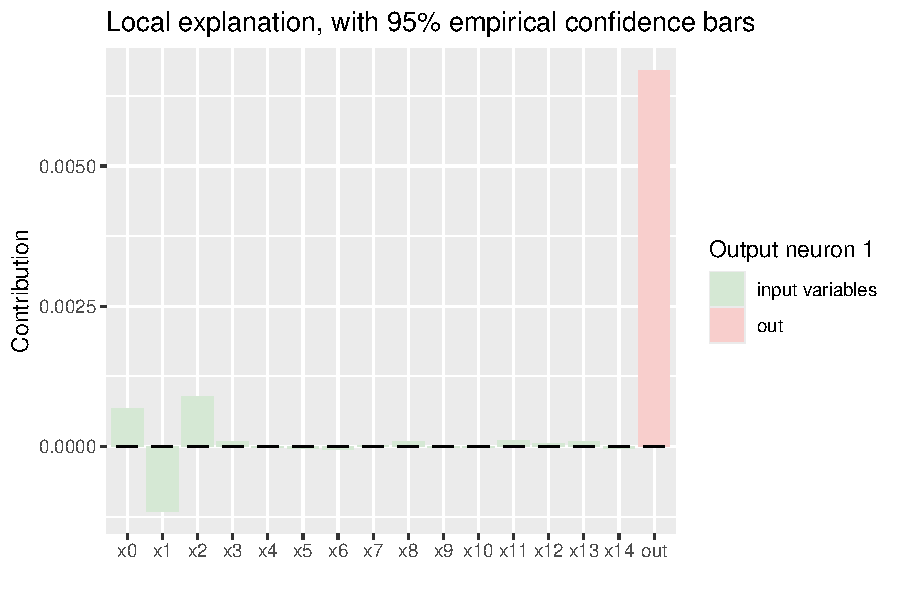
\includegraphics[width=0.6\textwidth]{figures/tut1_local.pdf}
    \caption{Local explanation pathways for a single prediction in the linear regression tutorial. The explanation is computed as the input gradient of the sparse feed-forward model.}
    \label{fig:tut1_local}
\end{figure}

\subsection{Tutorial 2: Nonlinear Binary Classification}
The nonlinear tutorial uses $n=1000$, $p=15$, and a response generated from logarithmic, cosine, interaction, and quadratic terms involving six active inputs. The response is dichotomized at the median and fit with a \((15,5,5,1)\) input-skip binary classifier. This script uses the default SIC penalty, \(\lambda=\log(n_{\mathrm{train}})\), with \texttt{epsilon\_1 = 1}, \texttt{epsilon\_T = 1e-5}, and \texttt{steps\_T = 200}. The global plot shows the thresholded feed-forward active paths found by the model.

\begin{figure}[h]
    \centering
    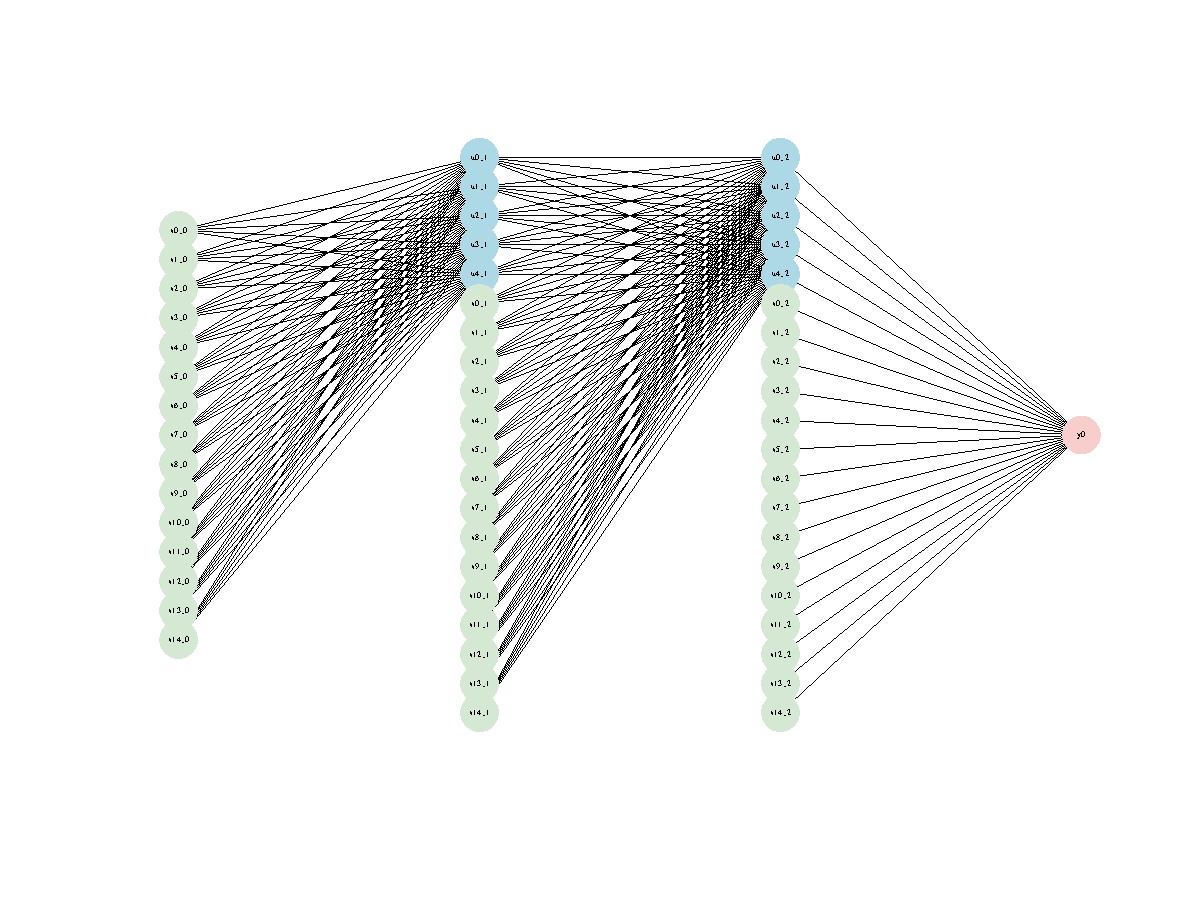
\includegraphics[width=0.8\textwidth]{figures/tut2_global.pdf}
    \caption{Global sparse structure for the nonlinear classification tutorial. Edges are retained when they are active under the SIC threshold and lie on an input-output path.}
    \label{fig:tut2_global}
\end{figure}

\subsection{Tutorial 3: Gallstone Classification}
The gallstone tutorial uses the packaged \texttt{Gallstone\_Dataset}, trains a \((40,3,3,1)\) input-skip binary classifier, and evaluates sparse prediction on a held-out split. The script uses the default penalty \(\lambda=\log(n_{\mathrm{train}})\), although \texttt{n\_train} is set to the full dataset size in the script rather than the size of the training split. The example demonstrates the intended workflow for tabular clinical classification: standardize inputs, train with SIC, validate both dense and sparse predictions, plot the global sparse graph, and compute local explanations.

\begin{figure}[h]
    \centering
    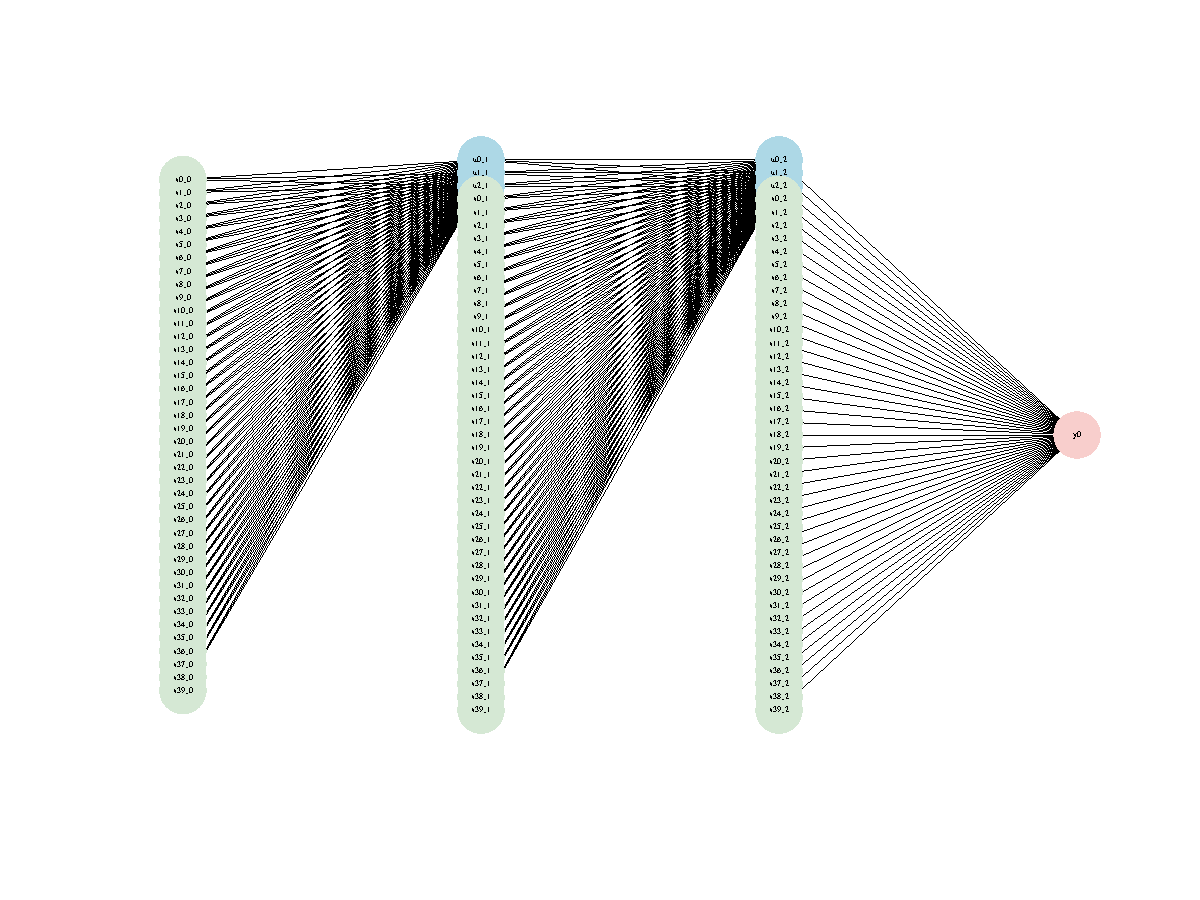
\includegraphics[width=0.7\textwidth]{figures/tut3_global.pdf}
    \caption{Sparse feed-forward pathways for the gallstone classification tutorial. The graph reflects thresholded active paths in an input-skip \texttt{SICNN\_Net}.}
    \label{fig:tut3_global}
\end{figure}

\subsection{Convolutional KMNIST Tutorial}
The KMNIST tutorial builds a two-convolution/two-dense classifier using \texttt{SICNN\_Conv2d} and \texttt{SICNN\_Linear}. It trains for one epoch by default and demonstrates that the SIC training loop, smooth parameter counts, sparse forward calls, and plotting method can be applied to the convolutional wrapper. This example should be read as an implementation and scalability demonstration. The current code does not compute active convolutional paths and does not establish exact spatial feature selection.

\subsection{LBBNN-Matched Experiments}
The repository also contains a separate set of deterministic SICNN experiments that reproduce the data-generating mechanisms, architectures, and fixed train/test splits used in the LBBNN study. These runs are not Bayesian comparisons: SICNN is fitted by the training objective described above, and all reported sparse models use deterministic active-path masking with $\phi_{\epsilon_T}(w)>0.5$. Some early binary discovery results in this subsection predate the classification-scale alignment described above; their stated penalties are on the earlier $-\ell$ scale and should be multiplied by two to reproduce the same objective with the current implementation. The repeated linear confirmation and Mice result use the current $-2\ell$ scale. Regression penalties are unchanged. This subsection records the best currently available fits and their settings, including limitations that should be resolved before treating them as a final benchmark.

\paragraph{Linear classification.}
For the LBBNN linear toy problem, $x_1,\ldots,x_4$ are generated independently from $\mathrm{Unif}(-10,10)$ before replacing $x_3$ by $\rho x_1+(1-\rho)x_3$. The binary response is the median split of $100+x_1+x_2+\varepsilon$, with $\varepsilon\sim N(0,0.01^2)$. A 10-seed paper-scale confirmation used $64{,}000$ training observations, $8{,}000$ test observations, a $(4,20,20,20,20,1)$ input-skip sigmoid network, Adam learning rate $0.002$, five mini-batches per epoch, 2,000 epochs, and a step scheduler at epoch 500. The SIC penalty was $80\log(n_{\mathrm{train}})$ and the epsilon telescope was $1$ to $10^{-5}$ over 200 steps. Median dense and sparse accuracy were both 0.999 at $\rho\in\{0,0.1,0.5\}$ (ranges 0.997--1.000, 0.998--0.999, and 0.999--1.000 respectively). These settings had median two active weights, true-positive rate one, false-positive rate zero, and exact-support rate one at all three correlation levels. At $\rho=0.9$, median dense and sparse accuracy were both 0.992 (0.988--1.000), with a median of three active weights; the mean false-positive rate was 0.35 and exact-support rate was 0.30. The result therefore confirms excellent prediction and exact support at low and moderate correlation, while retaining the expected redundant-feature ambiguity at high correlation.

\paragraph{Nonlinear classification.}
The nonlinear toy adds $x_1x_2+x_1^2+x_2^2$ to the preceding signal, while retaining the same four-input structure and correlated redundant $x_3$. The best discovery fit so far used $n_{\mathrm{train}}=n_{\mathrm{test}}=1{,}000$, a $(4,20,20,20,20,1)$ input-skip sigmoid network, 750 epochs, learning rate 0.005, a late step schedule at epoch 562, a $0.2\log(n_{\mathrm{train}})$ penalty, and an epsilon telescope from 0.1 to 0.005 over 100 steps. LBBNN-like structured initialization used scales 0.5 for hidden connections and 1 for covariate and direct-skip connections. This single fit achieved sparse and dense test accuracy 0.975 with 20 active weights and exact selection of $\{x_1,x_2\}$ at $\rho=0$. A partial three-repetition validation used a less aggressive $0.05$ to 0.005 telescope and penalties $0.125\log(n)$ and $0.14\log(n)$. Across $\rho\in\{0,0.1,0.5,0.9\}$, median sparse accuracy was 0.903--0.905 with median nine active weights; $x_1$ and $x_2$ were always selected, but exact-support rates ranged from 0 to 1/3. A subsequent 10-seed check at the current $-2\ell$ scale and $0.4\log(n)$ did not confirm this configuration: it frequently collapsed to very small, underperforming graphs. The nonlinear discovery result is therefore retained as a tuning observation only, not as a stable paper-scale benchmark.

\paragraph{Wisconsin Breast Cancer.}
The LBBNN split has 512 training and 57 test observations with 30 pre-scaled diagnostic inputs. Our current strongest repeated SICNN protocol used a $(30,50,50,1)$ input-skip sigmoid network, ten seeds (42--51), 500 SIC epochs, batch size 64, learning rate 0.01, a step scheduler at epoch 250, the current-scale penalty $\log(512)=6.238$, and an epsilon telescope from 0.05 to 0.005 over 100 steps. The SIC-selected active path mask was then locked, and the surviving weights and biases were refit on the training data for 100 unpenalized epochs at learning rate 0.01. This is a deterministic post-selection refit and does not alter the selected graph.

Before refitting, dense test accuracy had median 0.956 (range 0.930--1.000) and median AUC 0.997. The sparse-refit model had median test accuracy 0.965 (range 0.895--1.000), median AUC 0.997, median NLL 0.215, and a median of three active weights (range two to five) out of 5,580. The LBBNN repository reports median-probability accuracy 0.965 with a median of four active weights for this split, so the post-selection SICNN result now matches the headline accuracy and graph-size scale. The most frequently retained SICNN inputs were $x_{28}$ (8/10 runs), $x_8$ (7/10), and $x_7$ (6/10). Dense and sparse-refit metrics should be reported separately, since the refit is an explicit post-selection calibration step.

\paragraph{Abalone regression.}
For the LBBNN split of Abalone ($n_{\mathrm{train}}=3{,}759$, $n_{\mathrm{test}}=418$, $p=9$), the current strongest repeated SICNN protocol used a $(9,200,200,1)$ input-skip ReLU network over five seeds (42--46), batch size 751, 1,000 SIC epochs, learning rate 0.01, no learning-rate scheduler, penalty $0.5\log(3{,}759)=4.116$, and epsilon telescope 0.05 to 0.005 over 100 steps. Each SIC-selected active-path mask was locked, then the surviving weights and biases were refit for 100 unpenalized epochs at learning rate 0.01. This deterministic post-selection refit cannot alter the selected graph.

Before refitting, median dense test RMSE was 2.140 (range 2.113--2.159). The sparse-refit model had median RMSE 2.129 (2.069--2.153), correlation 0.783 (0.775--0.788), and 129 active weights (116--190) of 43,809. An affine calibration fitted on sparse training predictions gave median test RMSE 2.095 (2.070--2.124). This calibration is reported separately because it is an additional post-fit estimation step. All nine input features were retained in every run: the result is strongly edge-sparse but not feature-sparse. A paired seed-42 current-code control without refitting had affine-calibrated sparse RMSE 2.138 with 150 active weights, compared with 2.085 and 149 weights after refitting, supporting the interpretation that refitting improves estimation on a fixed selected graph.

To match the LBBNN hidden-layer nonlinearity more closely, we also fitted sigmoid networks. The best sparse sigmoid single-seed run with a multi-step schedule at 30\%, 50\%, 70\%, and 90\% of 1,000 epochs (decay factor 0.5), learning rate 0.02, penalty $0.05\log(3{,}759)$, and epsilon telescope 0.1 to 0.005 over 500 steps retained 133 weights and achieved test RMSE 2.210, correlation 0.758, and affine-calibrated RMSE 2.195. Thus the current predictive frontier favors ReLU, while the sigmoid result provides the direct activation-matched comparator and still needs a repeated sparse-refit evaluation.
\paragraph{Mice Protein Expression.}
The LBBNN repository supplies a fixed eight-class Mice Protein split with 972 training observations, 108 test observations, and 77 inputs. The repeated SICNN protocol used the LBBNN-shaped input-skip sigmoid architecture $(77,100,100,100,100,8)$, 2,000 epochs, batch size 36, learning rate 0.01, multi-step decay at epochs 1,000, 1,400, and 1,800 with factor 0.5, raw supplied inputs, an epsilon telescope from 0.05 to 0.005 over 500 steps, and a $0.2\log(972)=1.376$ penalty. Across ten seeds (42--51), median dense and sparse-refit accuracy were both 0.981 (ranges 0.972--0.991 and 0.963--0.991), with median balanced sparse-refit accuracy 0.981 and 112 active-path weights (108--121). The selected model retained a median of 60 inputs (55--63). The earlier seed-42 value of 0.991 matches the LBBNN-reported median accuracy, but the repeated SICNN median does not; it should therefore be reported as a promising but currently lower-performing repeated result rather than an exact benchmark match.
\subsection{Benchmark on UCI Datasets}
The UCI benchmark script trains standardized input-skip networks of the form
\[
(p,100,50,20,\mathrm{out})
\]
and compares sparse SICNN predictions against GLM or multinomial/logistic baselines and random forests. Unlike the default BIC setting, the script uses dataset-specific penalty multipliers \(\lambda=c\log(n_{\mathrm{train}})\), with multipliers ranging from 0.005 to 1.0 in the current file. The table below records the values in \texttt{uci\_experiments/final\_uci\_benchmarks.log}.

\begin{table}[h]
\centering
\begin{tabular}{l|c|c|c|c|r}
\hline
\textbf{Dataset} & \textbf{Type} & \textbf{SICNN} & \textbf{GLM} & \textbf{RF} & \textbf{Sparsity} \\
\hline
Pima & Classification (Acc) & 0.779 & 0.773 & 0.773 & 99.9\% \\
Sonar & Classification (Acc) & 0.690 & 0.690 & 0.381 & 100.0\% \\
Breast Cancer & Classification (Acc) & 0.956 & 1.000 & 0.993 & 99.9\% \\
Wine & Multiclass (Acc) & 0.972 & 1.000 & 0.972 & 99.8\% \\
Airfoil & Regression (R2) & 0.570 & 0.532 & 0.504 & 99.9\% \\
Yacht & Regression (R2) & 0.970 & 0.969 & 0.912 & 100.0\% \\
Concrete & Regression (R2) & 0.419 & 0.486 & 0.280 & 100.0\% \\
Abalone & Regression (R2) & 0.472 & 0.450 & 0.513 & 99.9\% \\
Boston & Regression (R2) & 0.381 & -0.220 & 0.351 & 99.9\% \\
\hline
\end{tabular}
\caption{Performance metrics from the current UCI benchmark log. Sparsity denotes the percentage of penalized weight parameters removed by the final SIC threshold. For regression, $R^2$ values are reported. Yacht hydrodynamics used a log-transformed target.}
\label{tab:uci_results}
\end{table}

\section{Practical Tuning Guidance}
\textbf{Penalty coefficient.}
For the native regression, binary, and multiclass losses, the default \(\lambda=\log(n_{\mathrm{train}})\) is on the classical \(-2\ell\) BIC scale and is a useful starting point. In sparse linear simulations it produced lower false-positive rates than validation-selected penalties. In noisier, smaller, or wider settings, stronger penalties are often needed for structural recovery. In the current examples, explicit penalties range from BIC-scale values to much stronger values such as \texttt{penalty = 80}.

\textbf{Epsilon schedule.}
The epsilon telescope controls when the surrogate starts behaving like a hard $L_0$ count. If $\epsilon$ decreases too quickly, weights can be pushed into regions with nearly zero useful gradient. A practical default is to let \texttt{steps\_T} span much of training, commonly 60--80\% of the epochs in larger benchmark scripts.

\textbf{Thresholding.}
The default threshold \(\tau=0.5\) on \(\phi_{\epsilon_T}(w)\) corresponds to retaining weights whose magnitude exceeds the final epsilon scale. Raising the threshold gives a stricter sparse graph; lowering it can recover weak but useful edges. The alternative \texttt{threshold\_type = "abs"} uses an absolute weight cutoff.

\textbf{Learning rate and scheduling.}
Because the method depends on separating useful weights from weights that should shrink toward zero, very small learning rates can lead to poor structural separation. The examples use Adam with learning rates between 0.001 and 0.01 and often use \texttt{scheduler = "step"}.

\textbf{Biases and parameter counts.}
Current SIC counts include weights but not biases. If bias terms are important for a scientific degrees-of-freedom calculation, this should be reported separately or handled by fitting with \texttt{bias = FALSE}.

\section{Local Explanations and Uncertainty}
For input-skip feed-forward models, local explanations are computed by temporarily using the raw output and differentiating it with respect to the input:
\begin{equation}
g_j(x)=\frac{\partial \mu(W,x)}{\partial x_j}.
\end{equation}
Sparse explanations use the active-path masked model. The \texttt{coef()} method aggregates these gradients over one or more observations and can optionally attach uncertainty estimates.

The uncertainty code approximates parameter covariance using a sandwich-style estimator for penalized models. Let \(I_0\) denote an empirical Fisher approximation from per-sample gradients of the data loss, and let \(H\) denote a curvature approximation that adds the nonnegative part of the smooth penalty Hessian,
\begin{equation}
\frac{\partial^2 \phi_\epsilon}{\partial w^2}
=
\frac{2\epsilon^2(\epsilon^2-3w^2)}{(w^2+\epsilon^2)^3}.
\end{equation}
The implementation clamps this penalty curvature below at zero before forming diagonal or block-diagonal covariance approximations. For diagonal covariance, the resulting form is
\begin{equation}
\widehat{\mathrm{Var}}(w_j)
\approx
\frac{I_{0,jj}}{H_{jj}^2}.
\end{equation}
For block-diagonal covariance, each parameter tensor is treated as a separate block and inverted independently.

The variance of a local explanation is then approximated by the Delta method:
\begin{equation}
\mathrm{Var}(g(W,x)) \approx J_g \Sigma_W J_g^T,
\end{equation}
where \(J_g\) is computed by automatic differentiation. This provides a scalable post-fit uncertainty heuristic for local explanations. It should not be interpreted as full post-selection inference for the graph-selection procedure.

\section{Known Limitations}
\begin{itemize}
    \item The BIC connection is approximate for neural networks because the selected sparse graph is adaptive and the parameterization is generally nonregular.
    \item The smooth parameter count currently includes weight tensors but excludes biases.
    \item Feed-forward active-path extraction is implemented; convolutional active-path extraction is not yet implemented.
    \item Multi-restart training is a local-search heuristic and does not guarantee a global SIC optimum.
    \item Some legacy documentation strings in the code still refer to variational inference or posterior draws, but current \texttt{train\_SICNN()} and \texttt{predict()} behavior is deterministic SIC training and deterministic forward evaluation.
\end{itemize}

\end{document}
